\addtocontents{toc}{\protect}
\section{\texorpdfstring{\MakeUppercase{radiative transfer models and observables}}{radiative transfer models and observables}}
\label{sec:sn-rt}

\counterwithin{figure}{section}
\counterwithin{table}{section}


\subsection{Methods} \label{sec:methods}

Here we describe the radiative transfer models we apply as post-processing to the three-dimensional hydrodynamic models described in Paper I. 


% ======================
% ======================

\subsubsection{Vertical Temperature Profile} \label{subsec:temperature-profile}

The disk models in Paper I were initialized isothermally by setting the sound speed according to the midplane temperature $\Tmid$ at the SN's radius in a \citet{SirkoGoodman03} disk.
Continuing the assumption of hydrostatic equilibrium we apply a Gaussian temperature profile in $z$ over the entire domain for each snapshot as follows:
\begin{equation}
\label{eqn:temp-profile}
    T(z) =
    \begin{cases}
	\Tiso & T>\Tmid \\
	\Tmid e^{- \frac{z^2}{2 H_T^2}} & \Tfloor < T < \Tmid \\
	\Tfloor & T<\Tfloor
    \end{cases}
\end{equation}
where $\Tfloor=2000$ K.
We could use simply $T_iso = T_mid$, but in practice we find that we need to allow for some flexibility in regions modified by the SN Gaussian in the initial conditions.
As such, we set $T_iso = (1+\epsilon) T_mid$, and find empirically that $\epsilon=1e-2$ gives acceptable results.
We find the temperature scale height $H_T=1.7\,H$ by root-solving for the profile from the midplane temperature to the effective temperature $\Teff$ using the Eddington approximation
\begin{equation}
	T = \left( \frac{3}{8} \tau + \frac{1}{2} + \frac{1}{4\tau} \right)^{1/4}\ \Teff.
\end{equation}
where we calculate $\tau$ using the Rosseland mean opacity given the vertical disk density profile.
This formulation allows us to bypass regions modified by the SN and only apply the disk profile to zones where the disk is unchanged.


% ======================
% ======================

%
%  Section on Light Curves
%
\subsubsection{Radiative Transfer Post-Processing} \label{subsec:rad-transfer}


We calculate the wavelength-dependent continuum intensity emerging from the hydrodynamic models via post-processing including attenuation from absorption and scattering processes along each column.
The cooling timescale is long compared to the dynamical timescale for our setup, so we can consider the gas to be adiatibatic since radiative losses are small.
We solve the following form of the radiative transfer equation,
\begin{equation}\label{eqn:RadTrans}
    \cos\theta \frac{1}{(\kappa_\lambda + \sigma_\lambda)\rho} \frac{dI_\lambda}{dz} = -I_\lambda + S_\lambda,
\end{equation}
where $\theta$ is the direction of propogation, $\kappa_\lambda$ is the opacity due to true absorption, $\sigma_\lambda$ is the scattering opacity, $\rho$ is the volumetric gas density, $I_\lambda$ is the radiation field's intensity, and $S_\lambda$ is the source function.
The presence of scattering calls for an effective source function that depends on the Planck function $B_\lambda$ and the mean intensity $J_\lambda$,
\begin{align}
    S_\lambda &= \frac{\kappa_\lambda B_\lambda + \sigma_\lambda J_\lambda}{\kappa_\lambda + \sigma_\lambda}  \nonumber\\
              &= (1-\omega_\lambda) B_{\lambda} + \omega_\lambda J_\lambda \label{eqn:effective_source}
\end{align}
where $\omega_\lambda = \sigma_\lambda / (\kappa_\lambda + \sigma_\lambda)$ is the single-scattering albedo.
The subscript $\lambda$ indicates quantities with wavelength dependence.
By restricting $\theta$ to be either 0 or $\pi$, we adopt the two-stream approximation which allows the radiation field to travel only upwards ($\Iplus$) or downwards ($\Iminus$), respectively, along the $z$-axis through independent columns of cells located at a given $(x, y)$ position.
First, we tried direct integration like in \citet{Godines+26}, but unlike a protoplanetary disk, an AGN disk is not isothermal and does not allow for this crude integration which could not capture the dependence of $S_\lambda$ on $J_\lambda$.
Therefore, each column is treated as an isolated stream and is solved using the Feautrier method \citep{Feautrier64,Cannon70}, an implicit method which calculates the mean intensity at each point simultaneously.
See Appendix \ref{sec:Apdx-Feautrier} for our modification of the method to include scattering and our boundary conditions.

\subsubsection{Opacities}
Given the density and temperature of a zone, we solve for the populations of neutral hydrogen H, ionized hydrogen $\Hplus$, the negative hydrogen ion $\Hminus$, and free electrons.
The neutral and negative ion species absorb radiation when an electron is stripped away through the bound-free (bf) ionization process, $\kappa(\text{H}_\text{bf})$ and $\kappa({\Hminus_\text{bf}})$ respectively, and the positive and negative hydrogen ions absorb photons via free-free (ff), or Bremsstrahlung, interactions with free electrons, noted as $\kappa (\text{H}_\text{ff})$ and $\kappa (\Hminus_\text{ff})$.
We calculate the combined continuous absorption from these processes, following \citet{Gray76,Gray21}, as
\begin{align}
	\kappa_\lambda =& \biggl\{ \bigl[ \kappa(\text{H}_\text{bf}) + \kappa(\text{H}_\text{ff}) + \kappa(\text{H}^-_\text{bf}) \bigr] (1 - 10^{-\chi \theta}) \nonumber \\
		    &+ \kappa(\text{H}^-_\text{ff}) \biggr\} \frac{1}{1 + \Phi_\text{H}(T) / P_\text{e}}  + \kappa(\text{e}^-).
\end{align}
The factor $1-10^{-\chi\theta}$ accounts for the stimulated emission of H and $\Hminus$ with $\theta = 5040 / T\ \text{eV}^{-1}$ and $\chi(\lambda) = 1.2398 \times 10^4 / \lambda\ \text{eV}$ when $T$ is in Kelvin and $\lambda$ is in \r{A}ngstr\"om.
The ionization state $\Phi_\text{H}(T)$ is given by the Saha equation, and $P_\text{e}$ is the partial pressure due to free electrons.
Though scattering processes in general can be wavelength-dependent, the scattering coefficient for free electrons $\sigma$ is wavelength-\emph{independent}, but it is proportional to the ratio between the number densities of ionized hydrogen $n_\text{HII}$ to total hydrogen $n_\text{H}$, $\sigma = 0.6648 \times 10^{-24} \,n_\text{HII} / n_\text{H}$.
This model ignores line opacities and only treats the continuum emission.
See Appendix \ref{sec:Apdx-Opacities} for full descriptions of the absorption and scattering coefficients.



\subsection{Results} \label{sec:results}

\subsubsection{Fiducial Model} \label{sec:fiducial-results}

The \citet{SirkoGoodman03} disk has the highest volume density at $10^3\,\Rs$ where we place our fiducial miplane model \code{r1e3-z0h}.
This location was also chosen because it is the most optically thick and thus most likely to prevent or delay electromagnetic radiation from reaching the disk photosphere.
Using \eq{eqn:temp-profile} to apply the temperature profile, we set $\Tmid=6\times10^4$ K.
The blue curve in Fig.~\ref{fig:all_lcs} is the light curve calculated using our post-processing radiative transfer code Ocotillo (see Appendix \ref{sec:Appendix-RTModel}) after integrating the flux over 50 wavelengths over the range $800\leq\lambda\leq8000\ \text{\AA}$.
The light curve remains constant for the first $\sim$20 days when the shock begins to pass through the disk's photosphere and breaks free at $\sim$30 days.
The luminosity rises to $10^{46}\,{\rm erg\,s}^{-1}$ over the next 50 days as the shock expands outside the disk, peaking at $\sim90$ days.
The kink in the light curve at this time is due to the shock crossing the $z$-boundary, meaning we do not capture the true peak of the lightcurve.

\begin{figure}[h]
    \begin{subfigure}{0.5\textwidth}
        \centering
        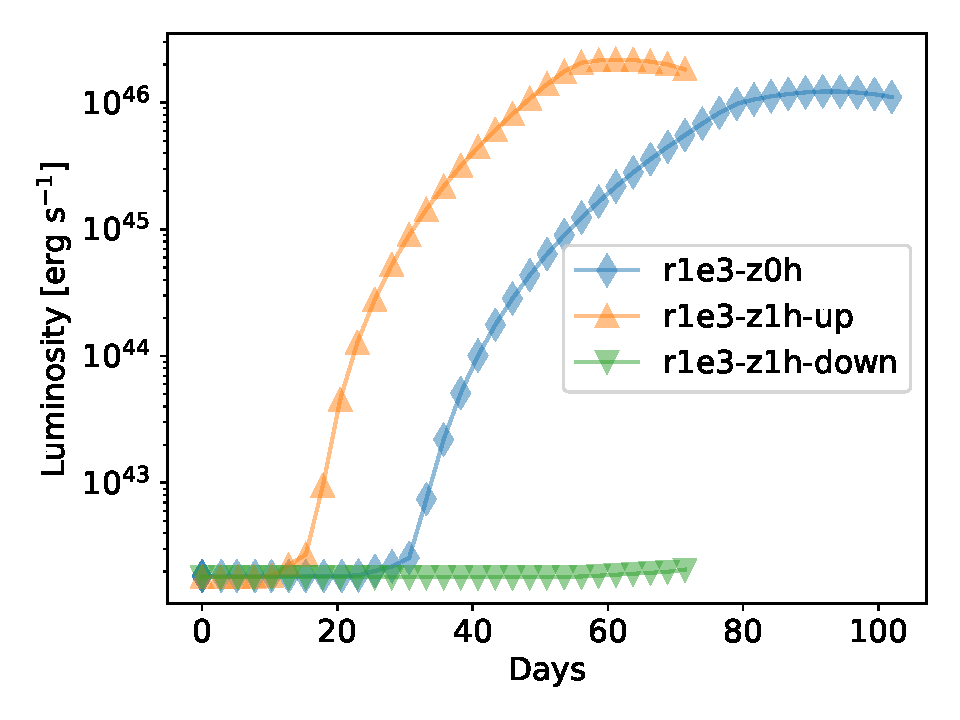
\includegraphics[width=1\linewidth]{ch4_figs/lightcurves_r3.pdf}
    \end{subfigure}
    \begin{subfigure}{0.5\textwidth}
	\centering
        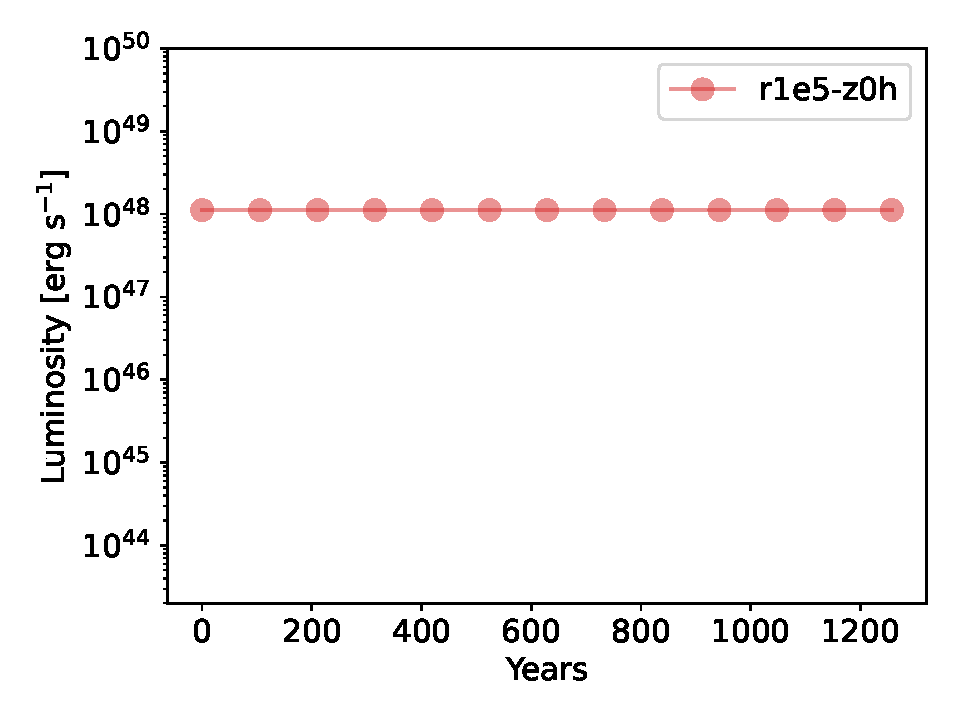
\includegraphics[width=1\linewidth]{ch4_figs/lightcurves_r5.pdf}
    \end{subfigure}
	\caption{Optical light curves for our SN simulations integrated over 50 wavelength bins spanning 800 to 8000 $\text{\AA}$.
	\code{r1e3-z0h} is our midplane fiducial model at $r=10^3\,\Rs$, \code{r1e3-z1h} is our model at the same radius but with the SN placed at a height $z=1\,H$.
	The curve labeled with \code{-up} is produced when observing from the positive $z$ boundary (i.e., the same side of the midplane as the offset SN), while the curve labeled with a \code{-down} is produced when observing from the negative $z$ boundary, or the far side of the disk.
	The lower pannel shows the lightcurve from our \code{r1e5-z0h} model which places a midplane SN at $r=10^5\,\Rs$.
    % The radiation from the midplane supernova (solid line) escapes the optically thick disk after $\sim$30 days, and the luminosity rises over the next 60 days and peaks at $10^{46}$ erg s$^{-1}$. 
    }
    \label{fig:all_lcs}
\end{figure}

\subsubsection{Offset Model}

Our model where the SN is placed at $z=1\,H$ produces two different light curves when viewed from opposite sides of the disk.
When viewed from the same side of the midplane as the SN (model \code{r1e3-z1h-up}) the green points show changes in the light curve occur earlier, corresponding to the shorter time it takes the shock to reach the disk photosphere.
Now, the radiation excapes at $\sim15$ days and rises faster than the midplane case in \code{r1e3-z0h} to a peak twice as bright.
Viewing from the far side of the disk (model \code{r1e3-z1h-down}), the orange points show no change at all with only a slight brightening when the flow reaches the disk photosphere near $\sim60$ days.

\subsubsection{SNe in the Outer Disk}

The bottom panel of Fig.~\ref{fig:all_lcs} shows the lightcurve for model \code{r1e5-z0h} were a midplane SN is placed at $r=10^5\,\Rs$.
In Paper I, the shock from this SN did not break free from the disk, and we see that the light curve similarily remains constant.
The baseline luminosity for the disk in this lightcurve is higher than the other light curves due to the hotter effective temperature of the disk at $r=10^5\,\Rs$. 

% Text for the color evolutions.
% The right panel shows the color evolution when comparing the central wavelengths in the $g$ and $r$ filter bands. The color becomes bluer as the bright shock dominates the dimmer disk. However, the color only changes by 0.04 -- well within the scatter of the ZTF data for AGN J1249$+$344.


\subsubsection{Color Evolution}
SNe are often classified and identified by their color evolution.
We integrate the flux emitted by our models over the wavelength ranges corresponding to the ZTF $g$ and $r$ band filters and calculate the $g-r$ color evolutions with:
\begin{align}
	F_{i} &= \int_{\lambda_{i}^0} ^{\lambda_{i}^1} F_\lambda d\lambda \\
	g-r     &= -2.5\log_{10}\frac{F_g}{F_r}
\end{align}

\Fig{fig:color-lightcurve} shows the color evolution for each of the models.
For models \code{r1e3-z0h} and \code{r1e3-z1h-up}, the color becomes slightly bluer when the hot shock emerges and remains constant as the ejected material expands.
Meanwhile, models \code{r1e3-z1h-up} and \code{r1e5-z0h} do not appreciably change color, mimicking their light curves, but \code{r1e3-z0h-down} does slightly change as the subsonic flow breaks through to the far side.
Even though two models showed color changes, the difference is small $\Delta (g-r)=0.04$ and would not have been detectable against the variability in AGN J1249$+$344 ($\Delta(g-r)\sim0.1$) if alert ZTF19abanrhr had been caused by a SN.

\begin{figure}
    \centering
    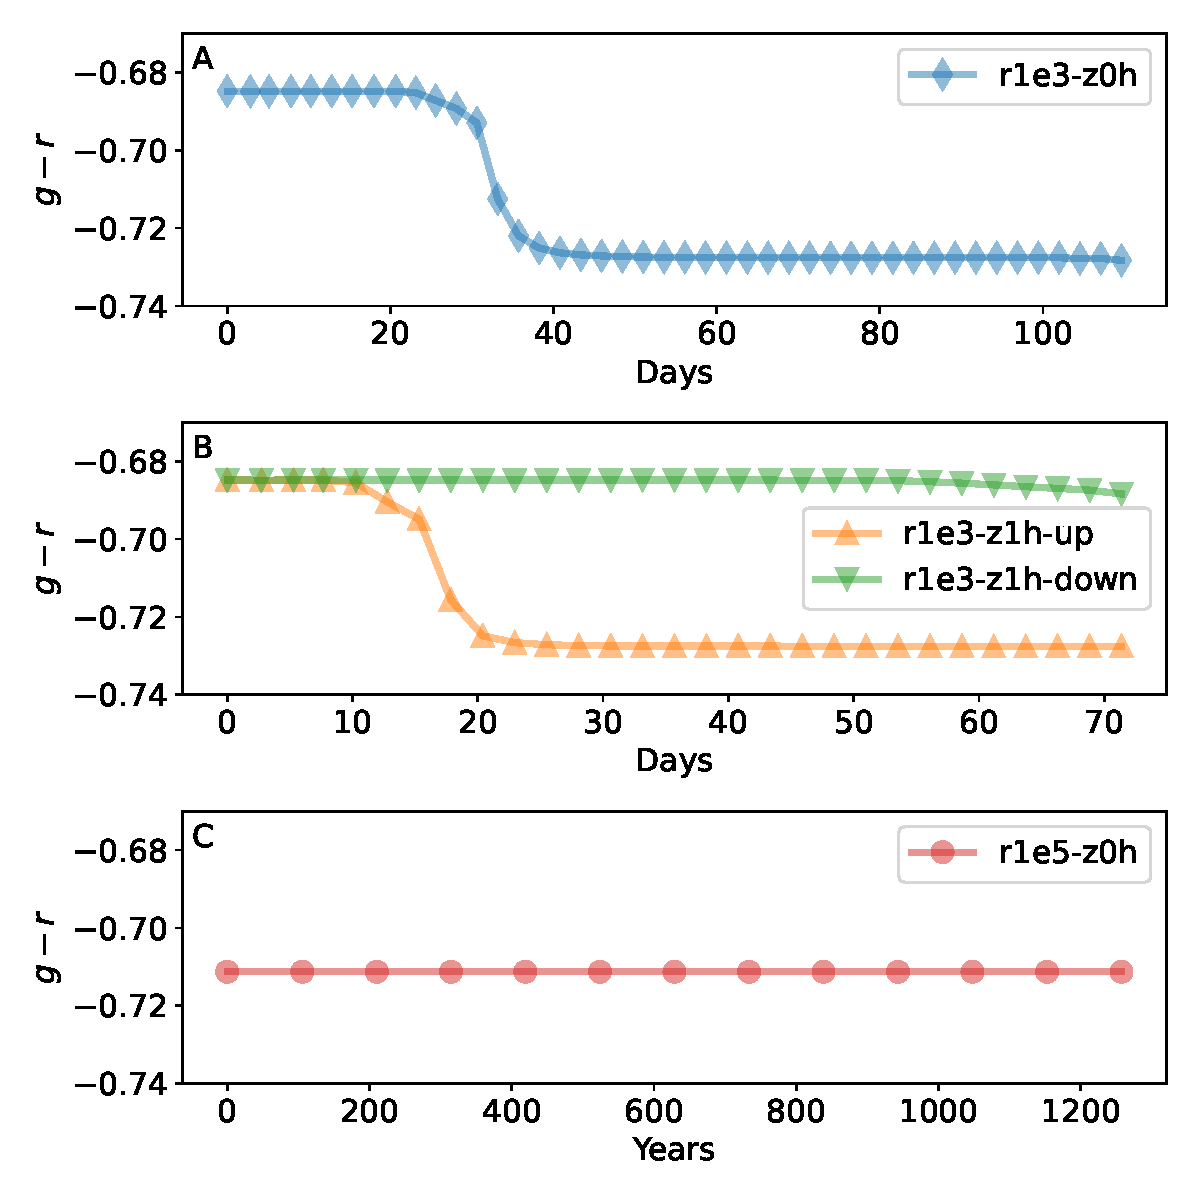
\includegraphics[width=1.0\columnwidth]{ch4_figs/gr_color_composite.pdf}
    \caption{ZTF $g-r$ color evolutions. Panel A is from our fiducial model at $R=10^3\,\Rs$, panel B is the offset model at the same radius, and panel C is the midplane model at $R=10^5\,\Rs$.
    The observed color becomes bluer when the shock breaks free, but the small change $\Delta(g-r)\sim 0.04$ would be undetectable amidst the noise for AGN J1249$+$344 with $\Delta(g-r)\sim0.1$ as reported by \citet{Graham+20}.}
    \label{fig:color-lightcurve}
\end{figure}


% \subsection{Magnitudes and Colors} \label{subsec:Mags+Colors}


% According to the methods described in the previous subsection, we derived a multi-wavelength flux $F_\lambda$ from our simulation. In order to compare them with the lightcurves quoted in \citet{Graham+20}, we convert the flux into apparent magnitudes.
% $F_\lambda$ is the value observed by a telescope placed directly at the z-boundary of the computational domain, so we convert these to apparent magnitudes for a source in AGN J124942.3 $+$ 344929 at $z=0.438$ or ~2.4 Gpc \citep{Graham+20}.

% To calculate a bandpass magnitude requires the zero point. ZTF filters are calibrated to match the Pan-STARRS 1 filters according to the release paper \citep{Bellm+19}. Magnitudes in this system follow the "monochromatic AB magnitudes" (Oke \& Gunn 1983)

% \begin{align}
% m_{\rm ABNU}(\nu) &= -2.5\log(f_\nu/3631\ {\rm Jy}) \\ 
%             &= -48.6 -2.5\log(f_\nu[{\rm erg/sec/cm}^2{\rm /Hz}])
% \end{align}
% \citet{Schlafly+12} reported zero points of $g_{\rm ZP}=24.41$ and $r_{\rm ZP}=24.68$, which we can use to calibrate the flux to those of the observations in \citet{Graham+20}.

\subsection{Discussion} \label{sec:discussion}

The baseline disk luminosities in Fig.~\ref{fig:all_lcs} are only produced by the radiation emitted by the small patch of the disk contained in the shearing box models, whereas the full integrated disk luminosity is much larger.
While studying spectra for AGN accretion disks, \citet{Hubeny+01} found that for a disk around a black hole of mass $\Mbh=10^8\,\Msun$ with a viscocity parameter of $\alpha=0.01$ has a luminosity $L=0.3L_\text{Edd}=4.4\cdot10^45(M/\Msun)$ erg s$^{-1}$ when considing electron scatting.
Therefore, only the SNe in models \texttt{r1e3-z0h} and \texttt{r1e3-z1h-up} may be detectable against the bright disk, and any observations would need to be able to distinguish changes from the disk emission by a factor of a few.

Additionally, as shown in \Fig{fig:color-lightcurve}, the color changes for these two SNe are very small ($\Delta g-r \sim 0.04$).



Comparing with alert ZTF19abanrhr, the proposed EM counterpart to GW190521, our lightcurves are similarly energetic, and exhibit the same lack of color evolution.
Therefore, an AGN-SN may be indistinguishable from a flare caused by the recoiling remnant of a BBH merger that creates a shock in the disk \citep{McKernan+19}. 
Future work should model the black hole recoil to identify distinguishing characteristics between the two events.

While the light curves do begin to level out, the peaks we see in the \code{r1e3-z0h} and \code{r1e3-z1h-up} curves in \Fig{fig:all_lcs} may be artificially caused by the shock passing through the $z$ boundaries.
Also, our radiative transfer model is limited to one dimension, and therefore cannot account for scattering at oblique angles to the line of sight.
As such, the mean intensity may change due to this effect, but we have performed these calculations with a face-on view of the disk which is expected to be the brightest viewing angle.
However, massive stars in the disk may not detonate as SNe at all.
The disk is a large reservoir of hydrogen fuel that continuously replenishes the star's supply if it is sufficiently embedded in the disk.
\citet{CantielloJermynLin21} showed that stars can reach masses of $M\approx300\,\Msun$, easily passing through the so-called pair-instability mass gap that spans $60\lesssim M \lesssim 160\,\Msun$ \citep{WoosleyHeger21}.
Stars that reach these masses will need to expell much more massive envelopes that could significantly delay their shock breakout from the disk or turn it into a subsonic flow entirely.
Thus massive stars that do finally fuse iron in their cores while embedded in an AGN disk will likely not evolve the same as those that lived their lives in the field away from such a plentiful resource.

%\begin{itemize}
%    \item observable against AGN disk luminosity? (draw line next to LCs?)
%    \item how do SNe impact broad line region (BLR) of AGN?
 %   \item Are repeated SNe required to physcally perturb the disk enough for the  BLR to change (check paper I for discussions of the broadline region)?
 %   \item can SNe create hot spots that result in BLR variability?
 %   \item rates of these SNe given the star formation rate in the outer disk \citep{SirkoGoodman03, DittmanMiller20} and disk capture \citep{Fabj20}. Need to consider that stars possibly evolve differently in AGN due to its large fuel reservoir \citep{Cantiello21}.
%\end{itemize}


\subsection{Conclusions} \label{sec:conclusion}

We performed post-processing radiative transfer calculations on hydrodynamic shearing box calculations of SNe embedded in AGN disks.
By implementing the Feautrier method we calculated the absorption and scattering processes caused by hydrodgen atoms and free electrons.

For SNe at the midplane in the inner disk ($r=10^3\,Rs$), the radiation emerges $\sim30$ days later and rises quickly to a peak at $L=10^{46}\ \text{erg s}^{-1}$.
Typical AGN luminosities can be $\mathcal{O}(10^{43}-10^{48}\ \text{erg s}^{-1})$, so these SNe will only be brighter than AGN of $L\ll10^{46}$, which is the range for Seyfert galaxies and other low-luminosity AGN, and will not be visible in quasars.
Radiation from a SN at the same location but offset from the midplane at $z=1\,H$ emerges 15 days earlier, rises much faster, and peaks at $2 \times 10^{46}\ \text{erg s}^{-1}$ when viewed from the same side of the midplane.
The radiation does not reach the other side of the disk in a detecable manner under this scenario.
While bright, these SNe may not be detectable against a bright AGN disk, but would be easily seen if occuring in a starved disk or during an episode of lower mass accretion rates.
For SNe detonating in the outer disk at $r=10^5\,\Rs$, the large scale height of the disk prevents the hot shock from emerging from the photosphere.

Embedded SNe do not exhibit a significant color evolution.
Without this key indicator that is common to naked SNe, they may be indistinguishable from flares produced by recoiling BBH merger remnants.
As such we will need to consider a different part of the spectrum or aspects of these transients to reliably distinguish between flares emitted by embedded merger remnants versus embedded SNe in transient searches and archives such as ZTF or LSST.

